\documentclass[11pt,a4paper,twocolumn]{IEEEtran}
\usepackage[utf8]{inputenc}
\usepackage[english,italian]{babel}
\usepackage{lipsum}
\usepackage{tabularx, booktabs}
\usepackage{amsmath}
\usepackage{amsfonts}
\usepackage{caption}
\usepackage{pdfpages}
\usepackage[margin=2.5cm]{geometry}
\usepackage{listings}
\usepackage{amssymb}
\usepackage{hyperref}
\usepackage{graphicx}
\usepackage{svg}
\usepackage{pgf}
\usepackage{array}
\usepackage{cancel}

\newcolumntype{L}[1]{>{\raggedright\let\newline\\\arraybackslash\hspace{0pt}}m{#1}}
\newcolumntype{C}[1]{>{\centering\let\newline\\\arraybackslash\hspace{0pt}}m{#1}}
\newcolumntype{R}[1]{>{\raggedleft\let\newline\\\arraybackslash\hspace{0pt}}m{#1}}


\author{Saverio Monaco\\ \sepline}
\title{\textbf{Risolutore di Flow}}

% \sepline dopo \maketitle rende tutto più carino
\newcommand{\sepline}{\noindent\makebox[\linewidth]{\rule{\textwidth}{1.2pt}}}
\newcommand{\bsepline}{\noindent\makebox[\linewidth]{\rule{7.5cm}{1.2pt}}}
\newcommand{\esepline}{\noindent\makebox[\linewidth]{\rule{7.5cm}{0.5pt}}}

\newcommand{\mysvg}[2]{\includesvg[width=0.#2\linewidth]{../svgs/#1}}

\newcommand{\code}[1]{\textbf{\texttt{#1}}}

\newcounter{algoritmo}
\setcounter{algoritmo}{1}
\newenvironment{algoritmo}{\bsepline\\{\large \code{Codice} \arabic{section}.\arabic{algoritmo}}\\ \bsepline}{\\\esepline\addtocounter{algoritmo}{1}}
\begin{document}
	\maketitle
	\selectlanguage{english}
	\begin{abstract}
		La funzione di questo programma è di risolvere i puzzle di tipologia simile a quella dell'applicazione \textit{Flow}, trovando tutte le soluzioni possibili. L'algoritmo è ispirato alla tecnica di Backtracking e, data la complessità computazionale del problema, si è cercato di lavorare principalmente sulla velocità di esecuzione a discapito della memoria.\\ Sono state inoltre implementate delle funzioni dedicate alla risoluzione degli esatti livelli dell'applicazione ufficiale e il gioco da terminale.
	\end{abstract}
	\selectlanguage{italian}
	\vspace{-.5cm}
	\section{Il puzzle}
	Flow è un puzzle logico nel quale il giocatore deve riuscire a connettere tutte le coppie in una griglia tramite percorsi, muovendosi nelle 4 direzioni e con la difficoltà che questi percorsi non possono intersecarsi.\\
	Nell'applicazione originale le coppie vengono distinte tramite colori, in questo articolo invece, per evitare un utilizzo eccessivo di colori e per rappresentare effettivamente come sono state salvate le informazioni in memoria, vengono usati dei numeri, in particolare la prima coppia è composta dai punti 1 e 2, la seconda dai numeri 3 e 4, e così via.\\
	Ad esempio:
	
	\begin{figure}[h]
		\hspace*{0.2cm}
		\mysvg{Numberlink_puzzle}{4}
		\mysvg{Rightarrow}{06}
		\mysvg{Numberlink_puzzle_solution}{4}
	\end{figure}
	
	\section{L'algoritmo risolutivo}
		\subsection*{L'algoritmo}
		Trovare la soluzione di un determinato puzzle di Flow è di complessità non polinomiale\footnote{\href{https://en.wikipedia.org/wiki/Numberlink\#Computational_complexity}{Numberlink - Wikipedia}}, per avere un'idea di ciò, si è riportato il calcolo del numero dei percorsi, di una coppia in una griglia quadrata di lato L, con i punti della coppia posti agli estremi della prima diagonale:\\
		\vspace*{-0.2cm}
		\begin{center}
		\begin{tabular}{|c|l|}
			\hline 
			\textbf{\quad L\quad } & \textbf{\# Percorsi} \\ 
			\hline 
			2 & 2 \\ 
			\hline 
			3 & 12 \\ 
			\hline 
			4 & 184 \\ 
			\hline 
			5 & 8512 \\ 
			\hline 
			6 & 1262816 \\ 
			\hline 
			7 & 575780564 \quad\\ 
			\hline 
		\end{tabular}
		\end{center}
	\begin{figure}[h]
		\qquad\quad\text{ }
		\centering
		\mysvg{npaths}{5}
	\end{figure}
    \vspace*{-1.6cm}
%\`{E} possibile ridurre il problema nella ricerca di una funzione capace di trovare tutti i percorsi possibili dato un punto di partenza ed un punto d'arrivo su una griglia in presenza di ostacoli (celle già occupate). Si dovrà infine riuscire a combinare questo algoritmo con tutte le coppie per trovare tutte le soluzioni complessive.
	Per la ricerca dell'algoritmo migliore si è ricorso all'approccio \textit{Divide et Impera}: si è scomposto il problema della ricerca delle soluzioni complessive nel problema della ricerca di tutti i percorsi delle singole coppie. Si troveranno quindi tutti i percorsi della prima coppia, e per ciascun percorso trovato si passa alla ricerca di quelli della seconda e così via.\\
%    Il problema della ricerca di tutte le soluzioni di un puzzle di Flow può essere scomposto nella ricerca di tutti i percorsi dato un punto di partenza, uno di arrivo e di celle già occupate: si cercano i percorsi per la prima coppia, e per ogni percorso trovato, si cerceranno le soluzioni della seconda e così via.\medskip\\
    Per trovare tutti i percorsi dato un punto di partenza e uno di arrivo è possibile considerare una struttura ad albero con ogni nodo rappresentante uno dei 4 movimenti possibili.
	\begin{figure}[h]
		\centering
		\footnotesize{\mysvg{tree1}{8}}
	\end{figure}
	\vspace{-3cm}\\
   Dal nodo iniziale (il punto di partenza) ci si potrà spostare nelle 4 direzioni, dopo di che il \textit{branching ratio} (il numero di nodi figlio per nodo madre) sarà al più di 3, perché tornare indietro non è uno spostamento possibile.\\
   Ovviamente non sempre tutte le 3 direzioni saranno disponibili, quindi il numero di nodi figlio potrà essere minore di tre fino a diventare 0 una volta che nessuna cella adiacente sarà libera.\\
   Muovendosi sui nodi dell'albero è possibile trovare tutti i percorsi possibili, il metodo scelto per esplorare l'intero albero in maniera ordinata è quello del \textit{Backtracking}, quindi seguendo le seguenti regole:
   Per trovare tutti i percorsi bisogna "muoversi" sui nodi dell'albero tenendo conto di tutti quelli visti in precedenza, il metodo scelto per fare ciò è quello del \textit{Backtracking}, ovvero seguendo le seguenti regole:
   \begin{itemize}
   	\item ogni volta possibile, si scende di un livello spostandosi nel nodo figlio più a sinistra disponibile;
   	\item se non è più possibile scendere di livello, si sale di uno e si prosegue nel nodo adiacente a destra.
   \end{itemize}
	
	Nell'\textit{Appendice A} viene mostrato come dovrebbe funzionare passo per passo l'algoritmo appena introdotto per un caso semplice di una griglia 3x3.\medskip\\
	
%	Trattandosi di un albero che si divide inizialmente in 4 nodi massimi, successivamente avente un branching ratio massimo di 3 e profondo al massimo 'base'$\times$'altezza' è possibile stabilire un massimo numero di nodi:
%	\begin{equation*}
%	\# nodi_{max}=4\cdot\left[\text{ }\sum_{i=0}^{b\cdot h-o-2}3^i\text{ }\right]
%	\end{equation*}
%	Dove b è la base, h l'altezza, o il numero di celle già occupate da altre coppie.\medskip\\
%	Questo valore orrisponde al numero di volte massime che la funzione chiamerà se stessa per singola coppia.\\
	Poiché ciascun nodo dell'albero può avere fino a 3 nodi figlio bisognerà trovare un modo per trovare e scartare quelli che non porteranno a nessuna soluzione, questi metodi si chiamano \textit{metodi di potatura dell'albero} e se vengono applicati a nodi poco profondi permettono di risparmiare un gran numero di chiamate a funzione.\medskip\\
	Per questo articolo è stato applicato solo un metodo di potatura dell'albero il quale verifica che durante la ricerca dei percorsi tutte le righe e colonne abbiano abbastanza celle libere da poter permettere il collegamento di tutte le coppie divise.\medskip\\
	Per chiarire il funzionamento di questo metodo si è portato un esempio:\\
	\vspace*{-.5cm}
	\begin{figure}[h]
		\centering
		\text{}\hspace*{0.5cm}{\large\mysvg{giacomo}{4}}
	\end{figure}\\
	Lo spostamento indicato in figura non porterà ovviamente a nessuna soluzione complessiva, poiché le coppie 3-4 e 5-6 dovranno entrambe passare da una singola cella. Evitare di compiere quella azione, farebbe risparmiare esattamente 155 mosse, e questo è solo uno dei tanti tagli che si possono applicare in questa stessa configurazione. In totale se si usa l'algoritmo per risolvere questo puzzle si dovranno fare 3311 mosse, mentre applicando questo metodo, se ne faranno solo 1037.\bigskip\\
	In sostanza si deve verificare che ogni riga e colonna abbia più celle libere che numero di coppie che esse hanno diviso.\\
	Per fare ciò bisogna utilizzare due array di interi, uno che controlla tutte le righe, e uno che controlla tutte le colonne, nella seguente maniera:
	\begin{enumerate}
		\item Si inizializzano i due array di interi:\\
		\begin{figure}[h]
			\vspace*{-.4cm}
			\centering
			\mysvg{expc/pcontrol1}{6}
		\end{figure}\\
		\vspace{-.5cm}
		\item Si da ad ogni valore dei due array, il numero di \underline{celle libere} della rispettiva riga o colonna:
		
		\begin{figure}[h]
			\vspace*{.0cm}
			\centering
			\mysvg{expc/pcontrol2}{6}
		\end{figure}
		\item A questo valore si sottrae il numero di coppie che la riga o colonna separa:
		\begin{figure}[h]
			\vspace*{.0cm}
			\centering
			\mysvg{expc/pcontrol3}{6}
		\end{figure}\\
		Il valore delle celle rappresenta il numero di celle che possono essere occupate in tale riga o colonna, senza che si incorra nel caso senza soluzione precedentemente descritto.\medskip\\
		\item Infine ogni volta che si cercano i percorsi per una nuova coppia, bisogna aggiungere '1' ad ogni cella dei due array relativi alla riga o colonna che ha diviso tale coppia perché durante le verifiche non si deve considerare la coppia corrente.
	\end{enumerate}
	Ad ogni spostamento bisogna aggiornare e verificare le celle relative alla posizione interessata, se uno dei valori diventa inferiore a '0', la mossa  non è valida: ci sarebbero meno celle libere, che coppie divise, che non potranno collegarsi.
		
	\iftrue
	\subsection*{Le strutture utilizzate}
	La funzione della ricerca dei percorsi si basa
	sulla tecnica del Backtracking che in codice corrisponde ad una funzione ricorsiva. Poiché questa
	funzione dovrà chiamare se stessa un gran numero
	di volte, è stato pensato di utilizzare variabili globali al fine di farne	 passare il minor
	numero possibile in input per non
	riempire immediatamente lo stack a funzione,
	cercando di lavorare sulla cache.\medskip\\ 
%	Avendo già premesso che il cuore dell'algoritmo consiste in una funzione ricorsiva, si è cercato di far passare meno variabili possibili di input. Per questo motivo tutte le strutture sono inizializzate come variabili esterne, quindi in particolare accessibile alla funzione ricorsiva senza bisogno di chiamarla.\medskip\\
	Le strutture adoperate sono:
	\begin{itemize}
		\item \texttt{int$^*$ \textbf{pgrid}}\\per rendere il codice più veloce è stato ritenuto migliore utilizzare un array di interi monodimensionale per rappresentare tutta la griglia.\\
		Le celle libere vengono salvate con l'intero '0', i due punti della prima coppia rispettivamente con gli interi '1' e '2', quelli della seconda coppia con gli interi '3' e '4' e così via.\\
		Una griglia costruita in tal modo però avrebbe l'ultima cella di una riga adiacente alla prima della successiva, quindi durante l'esecuzione dell'algoritmo si potrebbe incorrere a mosse errate in prossimità dei bordi, per ovviare a questo problema senza dover fare eccessivi controlli sulla posizione si è pensato di inizializzare l'array con un contorno di celle occupate, nella seguente maniera:
		\begin{figure}[h]
			\centering
			\qquad\qquad\quad\text{ }
			\mysvg{pgrid1}{35}
		\end{figure}
	\vspace*{-1.7cm}
			\begin{figure}[h]
		\centering
		\qquad\text{ }
		\mysvg{Downarrow}{03}
	\end{figure}
	\vspace*{-0.9cm}
		\begin{figure}[h]
	\centering
	\text{ }\hspace*{0.6cm}
	\mysvg{pgrid2}{6}
\end{figure}\\

	\(\bcancel{\fbox{\color{white}a}}\) rappresenta una cella di contorno,\\ {\fbox{\color{white}a}} rappresenta una cella libera della griglia.\medskip\\
	Inoltre per segnalare il contorno bisogna usare un valore intero non corrispondente a nessuno utilizzato per le coppie, perciò si è scelto '-1'.\\
	
	\item \texttt{int$^*$ \textbf{pcoppie}}\\ contiene le informazioni su i punti delle coppie, il primo intero indica il numero totale delle coppie, i restanti indicano la posizione dei punti delle coppie sulla griglia. L'array delle coppie serve sia a facilitare alcune funzioni secondarie (come la stampa), ma sopratutto per dire alla macchina da dove partire per trovare i vari percorsi durante la funzione ricorsiva.\\
	
	\item \texttt{int$^*$ \textbf{pcontrolx}$,$\space\textbf{pcontroly}}\\
	Sono gli array di interi con lo scopo di "potatura" dell'albero già introdotti. In base alle informazioni dentro questi array, è possibile predire se una mossa potrà portare o meno ad una soluzione complessiva.\\
	\end{itemize}
\subsection*{Le funzioni principali}	
	Con griglia e strutture già inizializzate, la parte principale dell'algoritmo risolutivo è composto da 3 funzioni principali:
	\begin{itemize}
		\item \code{flow\_risolutore()}:\\
		Lo scopo di questa funzione è inizializzare le strutture di controllo, impostare le variabili \texttt{numerosoluzioni} a '0' e \texttt{cursorecoppia} a '-1', in particolare quest'ultima funge da indice per l'array delle coppie \code{pcoppie} ogni volta bisogna cambiare coppia all'interno della ricorsione. Infine chiama la funzione \texttt{flow\_inizializzaprossimacoppia()}\medskip\\
		\item \code{flow\_inizializzaprossimacoppia()}
		Quando viene chiamata da \texttt{flow\_risolutore()} ed ogni volta che una coppia trova un percorso, viene lanciata questa funzione che aggiorna l'indice cursorecoppia passando alla coppia successiva. Prima di tutto viene fatto un controllo se abbiamo finito le coppie:\newpage
		\begin{algoritmo}
{\small		cursorecoppia+=2;\medskip\\
			/* Ci si chiede se non esistono altre coppie, in\\\text{  \space} caso si è trovata una soluzione complessiva */\\
			if(cursorecoppia $>$ (*(pcoppie)*2))\\
			\text{ }\{\\
			\text{ }\quad/* Si è trovata una soluzione */\\
			\text{ }\quad numerosoluzioni++;\medskip\\
			\text{ }\quad /* Si stampa la soluzione */\\
			\text{ }\quad flow\_grafica\_stampasoluzione();\medskip\\
			\text{ }\quad
			 /* Si torna alla coppia precedente */\\
			\text{ }\quad cursorecoppia-=2;\medskip\\
			\text{ }\quad return;}\\
			\text{ }\}
		\end{algoritmo}
	Nel caso in cui la coppia invece esiste, bisogna aggiornare le strutture di controllo come detto in precedenza e poi bisogna far partire la ricerca dei percorsi:
	\begin{algoritmo}
		{\small
		/* Si aggiornano le strutture al cambio di coppia */\\
		flow\_struttureausiliarie\_successivo();\medskip\\
		
		/* Si fa partire dalla ricerca dei percorsi nelle 4 direzioni,		ricordando che la griglia è un vettore di interi */	}\\
		{\small flow\_trovapercorsi(*(pcoppie+cursorecoppia)$-$riga);\\
			flow\_trovapercorsi(*(pcoppie+cursorecoppia)-1);\\
			flow\_trovapercorsi(*(pcoppie+cursorecoppia)+riga);\\
			flow\_trovapercorsi(*(pcoppie+cursorecoppia)+1);}
	\end{algoritmo}
	Poiché la funzione ricorsiva è sempre la stessa, viene ogni volta controllata anche la cella di provenienza; questo problema sarebbe potuto essere aggirato tramite la creazione di 4 funzioni ricorsive diverse anziché una, ma per mantenere semplice la stesura del codice si è scelta questa versione ad una funzione ricorsiva.\\
	Arrivato a questo punto del codice si sono esaminati tutti i percorsi per quella coppia dati i percorsi delle coppie precedenti, bisogna quindi ri-aggiornare le strutture di controllo e modificare \texttt{cursorecoppia}:\newpage
	
	\begin{algoritmo}
		{\small flow\_struttureausiliarie\_precedente();\medskip\\
		cursorecoppia-=2;}
	\end{algoritmo}
		\item \mbox{\code{flow\_trovapercorsi(int cursore)}}
		Il contenuto della cella sovrastante viene verificato solo dopo aver chiamato la funzione ricorsiva in tale cella, quindi all'inizio della funzione bisogna controllare se la cella interessata è una cella libera, occupata o quella che si sta cercando:
	\begin{algoritmo}
		{\small 
		/* Se la cella è libera... */\\
		if((*(pgrid+cursore))==0)\\
		\text{ }\{\\
		\text{ }\quad/* Si deve verificare se la mossa è lecita\\ \text{ }\quad tramite le strutture di controllo */\\
		\text{ }\quad if(!flow\_struttureausiliarie\_controllo(cursore))\\
		\text{ }\quad\{return 0;\}\medskip\\
	
		\text{ }\quad /* Se si è arrivati qui vuol dire che la mossa\\ \text{ }\quad è lecita */\\
		\text{ }\quad/* Si può occupare la cella, quindi scriviamo\\\text{ }\quad sull'array della griglia il numero giusto as-\\\text{ }\quad sociato alla coppia e aggiorniamo le strutture\\\text{ }\quad di controllo */\\
		\text{ }\quad *(pgrid+cursore)=cursorecoppia;\\
		\text{ }\quad flow\_struttureausiliarie\_aggiorna(cursore);\medskip\\
		\text{ }\quad /* Si lancia la stessa funzione nelle quattro\\ \text{ }\quad direzioni */\\
		\text{ }\quad flow\_trovapercorsi(cursore-riga);\\
		\text{ }\quad flow\_trovapercorsi(cursore-1);\\
		\text{ }\quad flow\_trovapercorsi(cursore+riga);\\
		\text{ }\quad flow\_trovapercorsi(cursore+1);\medskip\\
		\text{ }\quad /* Arrivato a questo punto della funzione\\\text{ }\quad bisogna segnalare libera la cella in questione*/\\
		\text{ }\quad *(pgrid+cursore)=0;\\
		\text{ }\quad flow\_struttureausiliarie\_riaggiorna(cursore);\medskip\\
		\text{ }\quad /* Non serve controllare gli altri casi */\\
		\text{ }\quad return;\\
		\text{ }\}\medskip\\
	/* Se la cella è quella che stiamo cercando... */
	if((*(pgrid+cursore))==(cursorecoppia+1))\\
	\text{ }\{\\
	\text{ }\quad flow\_inizializzaprossimacoppia();\\
	\text{ }\}
	}
	\end{algoritmo}
	Il caso in cui la cella è occupata e bisogna ritornare indietro è contemplato pure dal momento che nessun \texttt{if} andrà bene.
	\end{itemize}
	\section{Il gioco da terminale}
	Tramite la funzione\\ \code{flow\_game\_start(int base, int altezza, int numerocoppie)} è possibile giocare al gioco di flow, risolvendo un puzzle in una griglia 'base'$\times$'altezza' e con 'numerocoppie' coppie.\\
	Per creare un puzzle con soluzione si generano delle coppie con posizione casuale e si verifica se esiste soluzione, in caso contrario vengono ri-generate le posizioni delle coppie fino a quando non viene trovato un puzzle con almeno una soluzione. Ciò in codice si scrive:
	\begin{algoritmo}
		{\small\texttt{do\\\text{\space} \{\\\text{ }\quad\space inizializzagriglia(base,altezza);\\\text{ }\quad\space generacoppie\_rand(numerocoppie);\\\text{\space} \} while(!trovaprimopercorso())}}
	\end{algoritmo}
	\medskip\\
	Tramite una funzione simile a quella della ricerca dei percorsi, è possibile verificare se la soluzione immessa dall'utente è valida.
	\section{Conclusioni}
	Il programma creato riesce a risolvere tutti i livelli dell'app originale fin'ora provati in tempi relativamente brevi (il tempo più lungo registrato è stato 650 secondi), inoltre l'introduzione delle strutture di controllo porta nella maggior parte dei casi, una notevole diminuizione dei tempi di esecuzione. Per avere una idea di ciò, si è cronometrato il tempo di risoluzione di alcuni puzzle con e senza il metodo di potatura:\bigskip\\
	\hspace*{-.6cm}
	\begin{tabular}{|c|c|C{2.4cm}|C{2.4cm}|}
		\hline 
		Griglia & Coppie & Tempo senza potatura (s) & Tempo con potatura (s) \\ 
		\hline 
		9x9 & 10 & 8.27 & 1.06 \\ 
		\hline 
		9x9 & 9 & 35.91 & 1.20 \\ 
		\hline 
		9x9 & 8 & 465.73 & 7.42 \\ 
		\hline 
		9x9 & 7 & 5198.30 & 650.81 \\ 
		\hline 
	\end{tabular}\bigskip\\
	\`{E} chiaro quindi che l'introduzione di questo particolare metodo di potatura dell'albero delle mosse è stato un fattore determinante nella bontà complessiva del programma.\\
	Sarebbe possibile migliorare ulteriormente l'algoritmo nella risoluzione dei livelli dell'app sapendo che la soluzione finale prevede che tutte le celle siano occupate, quindi creando strutture ausiliarie apposite in modo da eliminare preventivamente tutte quelle mosse che portano a risultati invalidi.\\
	Per gli altri casi, se non si volessero trovare tutte le soluzioni esistenti, allora si potrebbero introdurre algoritmi euristici che potrebbero trovare un percorso in maniera più veloce.
	\clearpage
	
	\begin{appendices}
		\section*{\textbf{Appendice A}\\Algoritmo Step-by-Step}
		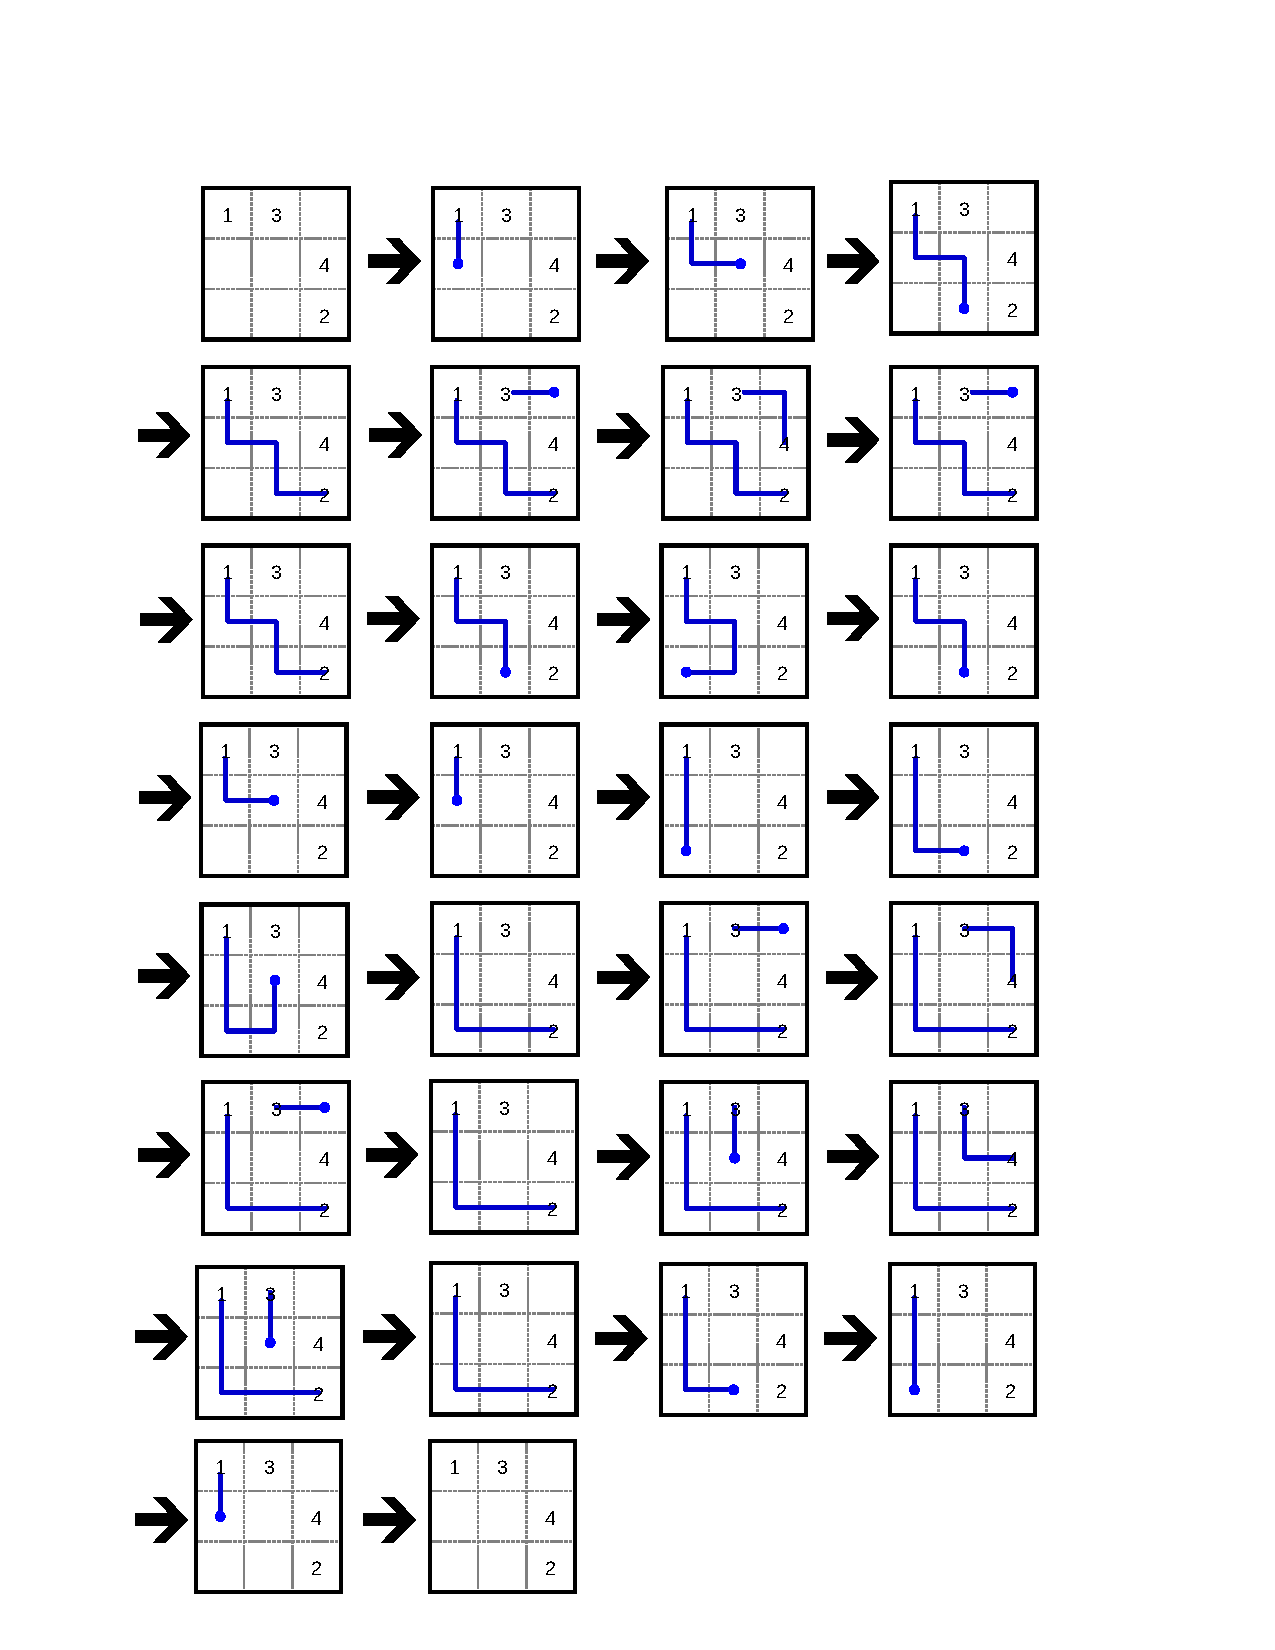
\includepdf[scale=1]{../svgs/algsbs/percorsipdf}
	\end{appendices}
	
\fi	
\end{document}


% https://en.wikipedia.org/wiki/Numberlink